\section{Méthodes et moyens mis en œuvre}
\label{sec:meth_moy}

Comme le titre l'indique, nous allons expliquer les méthodes et les moyens utilisés pour répondre à la problématique posée. Cette section sera séparée en 3 sous-sections : la première décrivant mon cheminement en matière de gestion de projet, la deuxième traitant de la phase de recherche d'informations, avec ses problèmes rencontrés et solutions trouvée, puis une troisième partie décrivant le travail effectué pendant la phase de test des deux produits sur un environnement de test, ainsi que toutes les différentes technologies utilisées.

\subsection{Gestion de projet}
\label{subsec:gestion}

La première chose que j'ai dû faire en arrivant dans l'entreprise, fut ce qu'on appelle chez \textsc{Synetis} une note de cadrage. Cette note de cadrage correspond, par rapport à ce qu'on a pu faire à l'université durant divers projets, à l'analyse des besoins et les résultats attendus, l'organisation en tâches de l'intégrité du stage. Cette répartition des tâches dans le temps a permis de scinder l'ensemble du projet en de multiples étapes simples, courte, qui m'a permis de segmenter mon stage pour ne pas me retrouver perdu ou submergé par le travail. En dernière partie furent explicités les contraintes et exigences de rendus pour l'entreprise ainsi que les éventuels risques à rencontrer.\\

\subsubsection{Analyse des besoins}
\label{besoins}
Le besoin général était de réaliser un état de l'art des solutions de gestion des comptes à privilèges, de mettre en place 2 preuves de concept sur un environnement de test virtualisé afin de pouvoir définir le ou les solutions les plus adaptés à la gestion des comptes privilégiés. Ces solutions pouvaient (à l'époque de la réalisation de l'état de l'art) et sont (à ce jour) déployés chez un gros client. Je suis notamment intégré à l'équipe travaillant sur cette intégration dans l'infrastructure, car ayant réalisé une mise en place dans un environnement de test de la solution en question, je fais parti des personnes les plus compétentes de \textsc{Synetis} pour répondre aux différents problèmes qui pourraient se présenter.\\
Cet état de l'art devait aboutir à un document présentant le principe de gestion de comptes à privilèges, premièrement de façon théorique, puis de façon technique. Ensuite, ce document devait faire une analyse d'une liste de solutions d'éditeurs étant des acteurs majeurs sur le marché de la gestion de comptes à privilèges. Enfin, ce document a aura permis de créer un tableau comparatif de toutes les solutions étudiées, selon des critères pointus qui ont été définis comme répondant à la problématique du stage.

\subsubsection{Planning prévisionnel}
\label{planning}
Afin d'avoir une vue d'ensemble du projet, un planning a été réalisé à partir d'un découpage journalier des tâches à effectuer. Ce planning a permis d'avoir une vue macroscopique du stage, et de répartir le travail sur la durée du stage, pour éviter d'avoir un retard qui pourrait surprendre à quelques semaines de la date buttoir. Ce découpage a aussi permis d'avoir des étapes, et de savoir à n'importe quel moment si j'avais de l'avance, ou surtout du retard, chose à proscrire pour arriver à un résultat convenable.\\
\begin{figure}[!ht]
    \center
    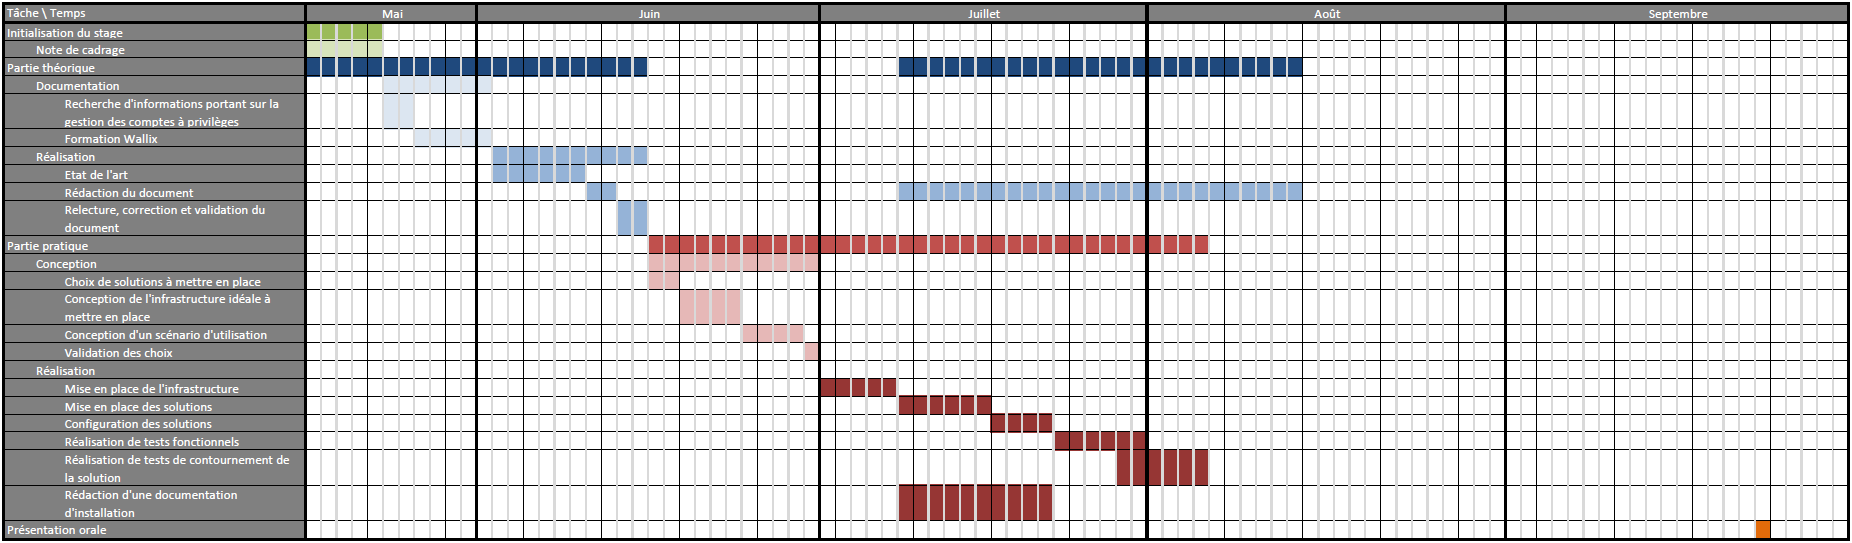
\includegraphics[width=\textwidth]{./images/calendrier_previsionnel.png}
    \caption{Calendrier prévisionnel}
\end{figure}

Bien sûr, le calendrier est une estimation et la réalité s'est avérée différente, ce point est abordé en section \ref{sec:resultats}. : la durée de recherche sur la gestion de comptes à privilèges et sur les différentes solutions a pris presque 2 fois plus de temps que prévu, tout comme le déploiement des solutions et le test de ces dernières. Cependant, le calendrier prévisionnel étant vu avec une large marge d'erreur, le stage tout de même pu être complété dans la durée impartie.

\subsection{Recherche}
\label{subsec:recherche}

La première étape a été la recherche d'informations sur le sujet. N'ayant pas de notions sur le sujet, j'ai d'abord commencé par me renseigner auprès des consultants de l'agence de Rennes, notamment mes tuteurs, Damien Seiler et Philippe Rolland, ainsi que le manager de l'agence, David Geffroy, ayant une base d'expertise dans le domaine. Grâce à ces premières lignes directrices fournis par ceux qui sont devenus mes collègues, j'ai pu orienter mes recherches internet vers la bonne direction, afin de trouver un maximum de résultats.

\subsubsection{Recherche du fonctionnement des solutions}
\label{par:fct_sol}
La meilleure façon de trouver des informations concernant le fonctionnement d'une solution de \gls{pam} s'est d'abord orientée vers la recherche d'informations génériques, comme des tutoriels ou des articles traitant du sujet. Cependant, j'ai fini par réaliser qu'il y avait très peu de ces ressources. La solution fut donc de directement s'orienter vers les solutions des éditeurs, et de tenter de comprendre leur fonctionnement, pour en tirer moi-même un fonctionnement général des solutions. Cette étape resta tout de même laborieuse, les éditeurs ne partageant pas énormément d'information quant à l'architecture ou le fonctionnement technique de leurs solutions, mais plutôt des caractéristiques de leur solution. Ceci ne m'empêcha pas de pouvoir trouver assez de solutions pour pouvoir en déduire une architecture assez claire, qui me donnait une vision d'ensemble du fonctionnement\footnote{Fonctionnement décrit dans un schéma en \textsc{Annexe} \ref{annexe:A}} d'une solution de \gls{pam}.\\

\subsubsection{Recherche des solutions existantes sur le marché}
\label{par:sol_market}
La recherche des solutions existantes sur le marché fut assez simple, compte tenu de la précédente recherche, s'appuyant sur ces solutions en question. Néanmoins, étant parti sur une base de 6 solutions trouvées pour réaliser un descriptif du fonctionnement général d'une solution de \gls{pam}, j'ai réussi à trouver plus du double de solutions par la suite, en navigant de lien en lien et en m'inscrivant à des newsletter m'envoyant des rapports tels que celui de l'éditeur \textsc{Forrester} écrit par Cser \cite{acs}.

\begin{figure}[!ht]
    \center
    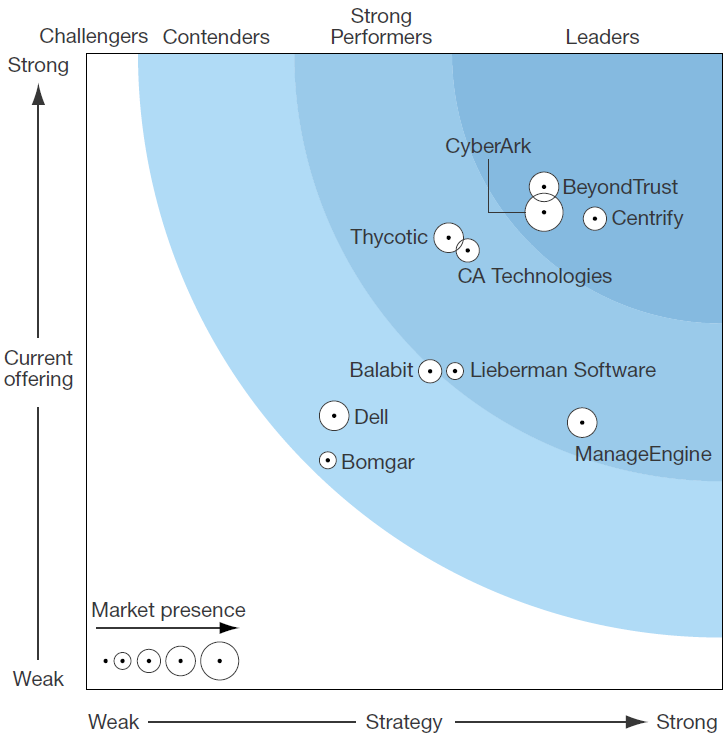
\includegraphics[width=0.7\textwidth]{./images/forrester_quadrant.png}
    \caption{Quadrant mettant en évidence les acteurs du marché de \gls{pam} selon le rapport offre/stratégie et l'indice de présence sur le marché}
\end{figure}

Nous avons ainsi pu nous retrouver avec une liste de solutions satisfaisante pour pouvoir commencer à faire un comparatif *réaliste* (terme à revoir). Nous avons alors orienté mes recherches vers les spécificités des solutions, en parcourant toute la documentation disponible, en participant à des vision-conférences avec les commerciaux et ingénieurs des maisons d'édition ou en contactant le support. Cette étape a été celle qui a pris le plus de temps dans la période de recherche, qui parfois s'est avérée infructueuse au vu du manque d'informations disponibles et de l'absence de réponse du support (ou plus précisément des réponses me redirigeant vers des documents en ligne ne contenant pas les réponses demandées). C'est par ailleurs une des étapes qui a complètement décalé le calendrier prévisionnel, prenant sur la marge prévue à cet effet.\\
Cette étape a conduit à éditer un tableau comparatif des solutions, dont nous pouvons trouver un aperçu à la \textsc{Figure }\ref{fig:tabcomp}. Ce tableau comparatif n'est pas disponible en annexe, à cause de sa taille impossible à imprimer, mais il reste tout de même disponible sur demande en format \emph{Microsoft Excel}.

\begin{figure}[!ht]
    \center
    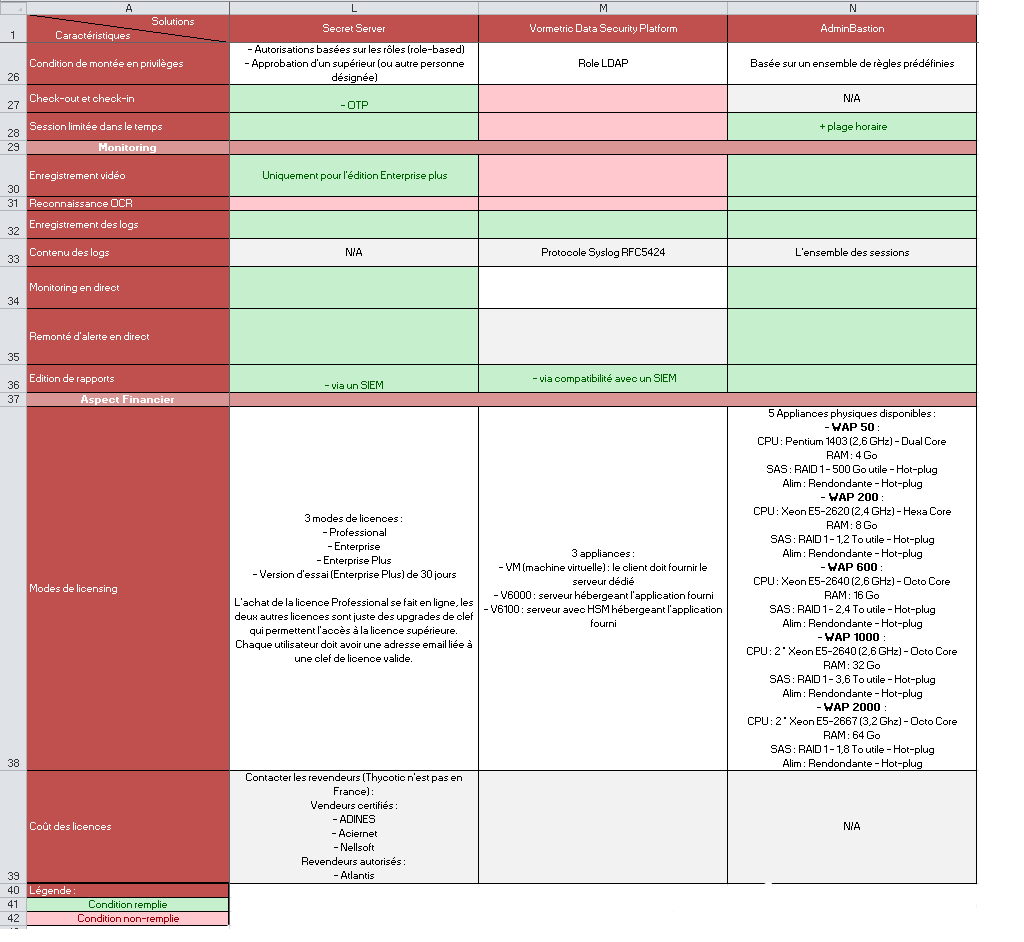
\includegraphics[width=\textwidth]{./images/tabcomp.png}
    \label{fig:tabcomp}
    \caption{Extrait du tableau comparatif de solutions édité au terme de la phase de recherche}
\end{figure}

\subsection{Proof of Concept}
\label{subec:poc}

La phase de conception d'environnement de test s'est déroulée en plusieurs étapes :
\begin{itemize}
	\item Conception architecture idéale
	\item Validation de l'architecture avec le tuteur, et remaniement de cette dernière pour s'adapter aux ressources matériels disponibles chez \textsc{Synetis}, ressources assez limitées car nous étions en saturation de ressources mémoire et processeur sur le serveur interne. Un nouveau serveur est arrivé en fin de stage, mais malheureusement quelques semaines trop tard
	\item Installation de l'infrastructure et déploiement des solutions à tester
\end{itemize}

\subsubsection{Architecture}
\label{par:archi}

L'architecture idéale sur laquelle les solutions devaient être intégrée nous semblait être celle qui se rapprochait le plus d'une situation réelle d'entreprise, comprenant des séparations logiques pour les différents corps de métier (

En effet, les ressources limitées ont réduit notre infrastructure de test au strict minimum, donc une machine de chaque type :
\begin{itemize}
	\item \textsc{MS Windows Server 2012 R2} : serveur de test de connexion RDP\footnote{Remote Desktop Protocol : contrôle à distance d'un serveur.}, de configuration des solutions de \gls{pam} (base de données \emph{MySQL} et \emph{SQL Server}), de mail (avec le logiciel \emph{hMailServer} \cite{hma} et contrôleur de domaine \emph{Active Directory}
	\item \textsc{MS Windows Server 2012} : serveur TSE\footnote{Terminal SErvice : permet d'utiliser le serveur pour faire tourner des applications utilisées en bureau distant.} permettant de tester une connexion sur une application distante (\emph{VMWare vSphere Client}\footnote{Programme Windows permettant de configurer un hôte de virtualisation et de faire tourner des machines virtuelles.} dans notre cas)
	\item \textsc{Linux Debian 8.4.0 Jessie} : serveur Linux permettant de tester une connexion SSH\footnote{Secure SHell : protocole de connexion à distance à une machine Linux/Unix.}
\end{itemize}

Cette architecture limitée nous a permis de tester et d'éprouver 2 des solutions choisies, tout en respectant les contraintes de ressources établies.\\
Bien plus que les solutions en elles-même, le déploiement de l'infrastructure de base a nécessité d'autres technologies, que l'ont peut lister en tâches suivantes :
\begin{itemize}
	\item Sur Microsoft Windows Server 2012 et 2012 R2 :
		\begin{arrowlist}
			\item Installation du rôle contrôleur de domaine\footnote{gestionnaire d'un domaine sous le système d'exploitation Windows.}
			\item Création et configuration d'un domaine, d'une forêt et de toutes ses dépendances assurant le bon fonctionnement de l'infrastructure
			\item Création d'utilisateurs de domaine\footnote{Utilisateurs créés dans un annuaire Active Directory, disponible pour toute machine du domaine.} avec les droits nécessaires et suffisant à leur fonctionnement, grâce aux groupes de sécurité Windows (consulter le livre de Minasi \emph{et al.} \cite{min} pour plus d'informations sur Active Directory et la sécurité de Windows Server 2012 R2)
			\item Création de comptes de service de domaine (MSA\footnote{Managed Service Account : compte Active Directory dédié aux service, le système gère lui-même les mots de passe.}) sous \emph{Powershell}\footnote{Interface en ligne de commande et langage de scripting dédié à Windows.}
			\item Installation de système de gestion de base de données relationnelle \emph{MySQL} et \emph{SqlServer} et création de bases de données pour les solutions de \gls{pam}
			\item Installation et configuration d'un serveur de mail local \emph{hMailServer} pour récupérer les mails envoyés par les solutions de \gls{pam}
			\item Installation du rôle TSE et configuration de ce dernier avec l'application \emph{VMWare vSphere Client}
		\end{arrowlist}
	\item Sur Debian 8.4.0 :
		\begin{arrowlist}
			\item Installation du serveur SSH
			\item Configuration réseau
		\end{arrowlist}
\end{itemize}

\subsubsection{Choix des solutions de \gls{pam} à tester}
\label{par:choixsol}

Nous avions fait, au terme de la phase de recherche, une sélection de 3 potentielles solutions à déployer sur nos environnements de test. Ce choix s'était fait en prenant en compte les données présentées dans le tableaux comparatif des solutions dont on a un aperçu dans la \textsc{Figure} \ref{fig:tabcomp}. Ces 3 solutions étaient :
\begin{itemize}
	\item \textsc{Wallix AdminBastion}
	\item \textsc{CyberArk Privileged Account Security Suite}
	\item \textsc{Thycotic SecretServer}
\end{itemize}

Nous étions déjà en contact avec \emph{Wallix}, car partenaires et mon tuteur était en train de passer une formation avec eux, pour la solution en question. Nous avons donc pu avoir facilement une installation de leur solution. En revanche, étant partenaire de \emph{Wallix}, \emph{CyberArk} a refusé de nous fournir une version d'évaluation tant que nous n'abandonnions pas notre partenariat, afin qu'il devienne notre partenaire exclusif. Ce choix de \emph{CyberArk} venant du fait que \emph{Wallix} est leur plus gros concurrent en France, car \emph{Wallix} est une entreprise Française et que beaucoup d'entreprises jouent le jeu de faire fonctionner une entreprise locale\footnote{Information fournie par le troisième éditeur, \emph{Thycotic} durant des échanges de mails.}. Nous avons donc décliné la solution de \emph{CyberArk} et sommes entrés en contact avec \emph{Thycotic}, avec qui nous n'avons pas eu de soucis et qui nous ont offert un suivi remarquable (une communication omniprésente à toutes les étapes de test).

\subsubsection{Déploiement : Wallix AdminBastion}
\label{par:depwallix}

La version d'essai de \emph{Wallix AdminBastion} se présente sous forme d'une machine virtuelle (fichier \texttt{vmdk}\footnote{VMWare Virtual Disk : format de disque virtuel créé par \emph{VMWare}}). L'hyperviseur\footnote{Plate-forme de virtualisation permettant de faire fonctionner plusieurs systèmes d'exploitation (dits virtualisés) sur une même machine physique.} hébergé sur le serveur local étant \emph{VMWare ESXi}, \\
Cette machine virtuelle est un Debian 8 personnalisé par Wallix, avec leur propre configuration d'usine. Elle doit utiliser une base de données \emph{MySQL} externe afin de stocker ses données (logs et accréditations). Nous avons donc créé une base de données sur le serveur \emph{MySQL} présent sur la machine Windows Server 2012 R2. On avait donc l'architecture présentée sur la \textsc{Figure} \ref{fig:archi_reelle}

\begin{figure}[!ht]
    \center
    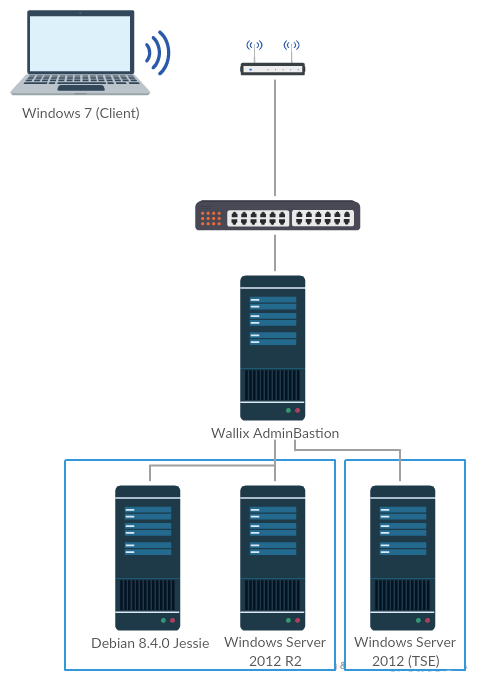
\includegraphics[width=0.7\textwidth]{./images/PoC_archi_reelle.png}
    \label{fig:archi_reelle}
    \caption{Architecture mise à l'échelle des ressources disponibles chez \textsc{Synetis}}
\end{figure}

Nous avons, suite à l'installation de la solution et à se configuration, pu tirer des points techniques important sur son fonctionnement. Le produit présente deux différentes interfaces, l'une étant hébergée sur le moteur même de la solution, que l'on appellera WAB et qui correspond au \gls{bastion}, l'autre étant beaucoup plus axée sur le design que l'on appellera WABAM\footnote{Wallix AdminBastion Administration Manager}, qui elle est hébergée sur un serveur parallèle, les utilisateurs de comptes à privilèges se connectent sur cette interface.\\

\paragraph{WAB}
Le WAB est le moteur central de gestion des connexions entre les ressources et les utilisateurs. C'est à partir de cette interface que sont gérés (ajout/suppression/modification) les utilisateurs de comptes à privilèges. Le principe de fonctionnement du WAB peut être décomposé en 4 parties :
\begin{enumerate}
	\item Les comptes utilisateurs, ils peuvent être locaux ou directement importés d'un annuaire LDAP, ce que nous avons fait pour le PoC, avec notre domaine Active Directory.
	\item Les ressources, qui fournissent des informations sur la localisation (adresse IP ou FQDN\footnote{Fully Qualified Domain Name : nom de domaine complet permettant de cibler une machine ou un équipement}) de cette dernière.
	\item Les comptes de ressource, avec les mots de passe qui peuvent être modifiés automatiquement grâce à une extension native ou programmable manuellement, qui sont les comptes des ressources précédemment citées.
	\item Les autorisations, qui font le lien entre les utilisateurs et les ressources (via leurs compte de ressource).
\end{enumerate}

\paragraph{WABAM}
Le WABAM est simplement une interface web qui récupère les informations que lui fourni le WAB. C'est une interface complètement personnalisable, sur laquelle se connectent les utilisateurs finaux. C'est une interface beaucoup plus élégante destinée aux utilisateurs finaux, qui est en fait une vitrine du WAB. Elle embarque des extensions permettant d'ouvrir une connexion RDP, SSH ou tout autre connexion disponible avec le WAB directement dans le navigateur web. Nous ne nous intéresserons pas plus à cette interface qui n'a pas beaucoup de valeur autre que son design et la séparation de l'administration des utilisateurs finaux.

\subsubsection{Test : Wallix AdminBastion}
\label{par:testwallix}

Une série de tests fonctionnels ont été effectués, des scénarios d'utilisation ont été joués : des connexions d'utilisateurs à des ressources, de toute origines possibles et sur un maximum de ressources disponibles (soit du RDP sur Windows, du SSH sur une machine Linux et une application sur un serveur TSE). Tout ces tests fonctionnels se sont relevés concluants.\\
Par la suite, nous avons recherché des points de faiblesse qui permettraient de mettre la solution en porte-à-faux. Certains points ont été trouvés, mais ces points nécessitent un non-respect des conseils de sécurité proposés par Wallix. Les points de faiblesse sont les suivants :
\begin{itemize}
	\item Single Point Of Failure\footnote{SPOF : point unique de défaillance, c'est un point unique dont tout le système d'information est dépendant.} : toutes les connexions passent par le WAB, on peut donc imaginer une attaque de type DDoS\footnote{Distributed Denial of Service : déni de service réparti (ou distribué), est une déni de service entraîné par une énorme masse d'information créant une congestion (le célèbre \texttt{ping flood} lancé depuis plusieurs machines est un DDoS).} bloquant le fonctionnement du WAB. Cependant, Wallix conseille d'éviter de mettre en place un système de haute disponibilité (deux machines WAB en parallèle qui traitent les requêtes), mais de plutôt monter un plan de reprise d'activité, qui consiste à conserver un serveur clone inactif en parallèle du premier, qui prendrait le relais en cas de panne et/ou attaque de ce type. Il reste aussi difficile de tenir une telle attaque dans la durée compte tenu de la quantité de ressources nécessaires. Enfin, le WAB ne devant être autorisé de l'extérieur du réseau (pour des prestataires par exemple) que depuis des adresses IP spécifiques, cette nécessité de ressources pour monter une attaque est encore moins atteignable.
	\item Contournement des routes : nous avons imaginé qu'un utilisateur modifie manuellement sa table de routage pour accéder directement aux ressources. Cependant, cette action nécessite deux prérequis :
	\begin{enumerate}
		\item Les ressources sont dans le même sous-réseau que les utilisateurs, ce qui est une très mauvaise pratique en terme de sécurité, car il est important de cloisonner les différents types de machines (serveurs/utilisateurs).
		\item Les mots de passe ne sont pas gérés automatiquement par le WAB, mais par des administrateurs, ce qui est totalement à l'opposé du but de l'utilisation d'une solution de PAM.
	\end{enumerate}
	\item Le vol d'une session d'un utilisateur, s'il part par exemple en pause et oublie de bloquer sa session. Mais cette faille est une faille humaine à laquelle on ne peut pallier uniquement en sensibilisant le personnel.
\end{itemize}

\subsubsection{Déploiement : Thycotic Secret Server}
\label{par:depss}

Encore une fois, l'architecture de l'infrastructure de test a été limitée par les ressources internes. La solution de \gls{pam} a dû être déployé sur le contrôleur de domaine Active Directory, ce qui n'est pas conseillé, car Windows Server gère très mal le cohabitation avec le rôle contrôleur de domaine et le rôle Internet Information Services (IIS).\\
La première tentative d'installation fut infructueuse, sûrement à cause de la machine qui avait déjà été utilisée pour un projet portant sur une autre problématique. Toute l'installation s'est bien déroulée (installation des rôles et sur SQL Server), mais une fois l'installation terminée, il était impossible de joindre le serveur "Secret Server" dans les pools d'application IIS (piscine d'applications). Le problème ne pouvant être résolu, même avec l'aide du support Thycotic, nous avons décider de repartir de zéro et de formater notre serveur, pour y ré-installer un serveur neuf, sans possible paramétrage générant des erreurs.\\
Cette seconde installation posa juste un soucis avec l'attribution des droits d'exécution, ne fonctionnant pas avec un compte de service\footnote{A partir de Windows Server 2008 R2, Microsoft à mis en place les MSA (Managed Service Account) afin de déléguer la gestion d'un compte de service à un domaine Active Directory. Ces compte n'ont pas de mot de passe attribué par un administrateur, mais ils sont tout simplement assigné à des machines qui ont le droit de récupérer ce mot de passe d'accès auprès du contrôleur de domaine. Ainsi il peut être modifié régulièrement sans affecter l'utilisation.}. Ce problème était sûrement dû à la cohabitation des rôles de contrôleur de domaine en même temps que le rôle IIS.\\
Du point de vu du routage, le Secret Server doit être positionner en proxy pour capturer les connexions et pouvoir les surveiller. En étant configuré dans ce mode, il permet d'établir toutes les connexions disponibles (SSH, RDP, Citrix, etc) directement dans le navigateur web.\\
Cependant, toutes ces configurations sont laborieuses à mettre en place, surtout si l'on a installé le logiciel en français (c'est peut-être aussi le cas pour les autres langues), car il est impossible de changé de langue une fois le logiciel installé, et donc de migrer vers la langue d'origine, l'anglais. La version française est très mal faite car les traductions sont très souvent fausses, il est donc compliqué de retrouver les configurations décrites dans le manuel. Par exemple, \og Edit Discovery Sources \fg{} traduit en \og Editer les Domaines \fg{} au lieu de \og Editer les sources de découverte \fg{}, sans parler des erreurs d'orthographe comme \og Déconnection \fg{} au lieu de \og Deconnexion \fg{}, qui n'influe pas sur la fonctionnalité, mais donne une très mauvaise image du sérieux que l'entreprise pourrait avoir.

\subsubsection{Test : Thycotic Secret Server}
\label{par:testss}